\section{Artificial neural networks} % (fold)
\label{sec:artificial_neural_networks}
% What is it
Artificial neural networks are models that can approximate discrete-valued, real-valued and vector-valued functions.
They are composed of simple units that can be activated by other units and can further activate multiple other units using connections of varying strength.
%citation?
Artificial neural networks are loosely inspired by biological neural networks, where these units are called neurons, which are connected by axons.\\
The higher the strength, also called weight, between units, the more influence the unit has on the connected one. These strengths can be manually defined. However, thanks to a method called backpropagation, these weights can be learned systematically. The combination of artificial neural networks and backpropagation led to successful applications, for example to recognize handwritten characters \citep{journals/neco/LeCunBDHHHJ89}, for face recognition \citep{cottrell1990extracting} and to recognize spoken words \citep{journals/nn/LangWH90}. However, they were also used for reinforcement learning, for example to learn to balance a pendulum \citep{anderson:ieeecsm89} or play Backgammon \citep{Tesauro:92}.

\subsection{Basics} % (fold)
\label{sub:basics}
As said, artificial neural networks are made up of units. These units can be divided into layer, where the values of each layer are propagated to the next layer depending on connections with weights. These weights define the model. A simple artificial neural network is visualized in Figure~\ref{fig:ann}.
\begin{figure}[htb]
    \centering
    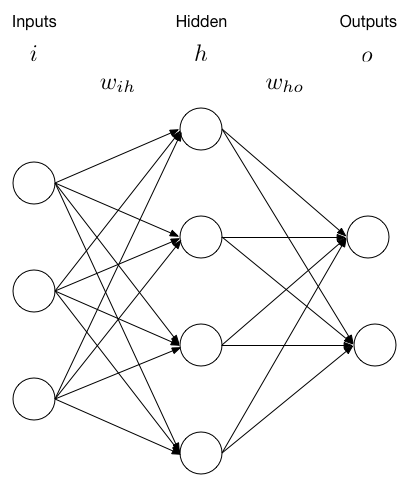
\includegraphics[width=.7\linewidth]{images/ann.png}
    \caption[An artificial neural network]{An artificial neural network with 3 input units, 4 hidden units and 2 output units. $w_{ih}$ and $w_{ho}$ are the weights for connections between respectively the input units and hidden units and between the hidden units and output units.}
    \label{fig:ann}
\end{figure}
% subsection basics (end)

% Inspired by biology
% Applications
% Activation functions
% (Stochastic) gradient descent
% Back propagation
% section artificial_neural_networks (end)